\documentclass{beamer}

\usepackage[slovene]{babel}
\usepackage[utf8]{inputenc}
\usepackage[T1]{fontenc}
\usepackage{lmodern}
\usepackage{amsmath, amsfonts}

\usetheme{Berlin}
\usecolortheme{default}
\useinnertheme[shadows]{rounded}
\useoutertheme{infolines}
\usepackage{array}
\usepackage{tikz}
\usetikzlibrary{arrows}
\usetikzlibrary{matrix}
\usepackage{graphicx}
\beamertemplatenavigationsymbolsempty

\usepackage{palatino}
\usefonttheme{serif}

\begin{document}

\title{Madžarska metoda}
\subtitle{Projekt}
\author{Borut Zupan}
\institute[FMF] {Fakulteta za matematiko in fiziko}
\date{2.6.2022}

%==========================================================
\begin{frame}
\titlepage
\end{frame}

%==========================================================
\begin{frame}
\frametitle{Opis}
    \begin{block}{}
        Madžarska metoda je:
        \begin{itemize}
            \item kombinatorni algoritem za optimizacijo,
            \item razvil Harold Kuhn,
            \item rešuje problem dodelitve,
            \item polinomski čas,
            \item najslabši primer je $O(n^3)$.
        \end{itemize}
        \hfill \break

        Problem dodelitve je:
        \begin{itemize}
            \item poseben primer transportnega problema,
            \item število ponudnikov $=$ število potrošnikov,
            \item količine ponudbe in povpraševanja so $1$.
        \end{itemize}
    \end{block}
\end{frame}

\begin{frame}
\frametitle{Graf}
    \begin{block}{} 
        Predstavitev z grafom:
        \begin{itemize}
            \item dvodelni graf ponudnikov in potrošnikov,
            \item količine so $1$, zato na vozliščih ni uteži,
            \item uteži na povezavah predstavljajo ceno storitve.
        \end{itemize}
    \end{block} 
\end{frame}

\begin{frame}
\frametitle{Primer grafa}
    \begin{figure}[htbp]
        \centerline{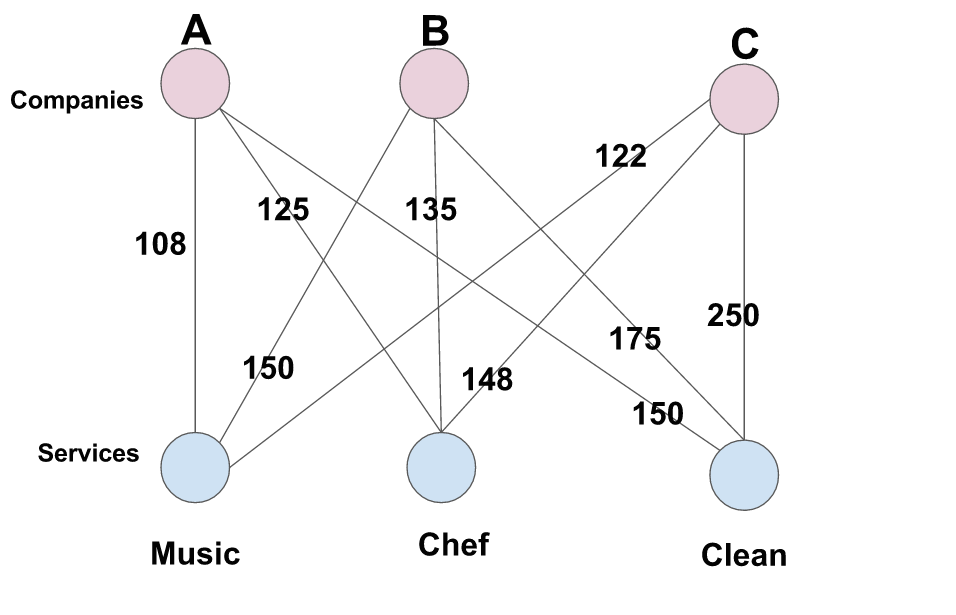
\includegraphics[scale=0.25]{bipartite_graph.png}}
    \end{figure}  
\end{frame}

\begin{frame}
\frametitle{Metoda}
    \begin{block}{} 
        Madžarska metoda je sestavljena iz dveh delov:
        \begin{enumerate}
            \item redukcija na vrsticah in stolpcih matrike
            \item rešitev optimiziramo na
            iteracijski način
        \end{enumerate}
    \end{block}
    \begin{block}{} 
        Madžarska metoda deluje, ker prištevanje ali odštevanje konstante vrstici
        ali stolpcu ne spremeni optimalne reštive.
    \end{block}
\end{frame}

\begin{frame}
    \frametitle{1. korak}
    \begin{block}{}
        Vsaki vrstici odštej nejn minimalen element. 
        (Če hočeš lahko narediš enako tudi za stolpce). Pojdi na 2. korak.
    \end{block}
    \hfill
    \begin{columns}[t]
        \begin{column}{0.25\linewidth}
         $\begin{bmatrix}
              1 & 2 & 3\\
             2 & 4 & 6\\
             3 & 6 & 9\\	
         \end{bmatrix}$
        \end{column}
        \begin{column}{0.005\linewidth}
         \centering
         $ \rightarrow $
        \end{column}
        \hfill
        \begin{column}{0.25\linewidth}
            \centering
            $\begin{bmatrix}
                0 & 1 & 2\\
                0 & 2 & 4\\
                0 & 3 & 6\\	
            \end{bmatrix}$
        \end{column}
    \end{columns}
\end{frame}

\begin{frame}
    \frametitle{2. korak}
    \begin{block}{}
        Najdi ničlo. Če v njeni vrstici ali stolpcu ni nobene ničle z zvezdico
        potem jo označi z zvezdico. To naredi za vsako ničlo.
    \end{block}
    \hfill
    \begin{columns}[t]
        \begin{column}{0.25\linewidth}
            $\begin{bmatrix}
                0 & 1 & 2\\
                0 & 2 & 4\\
                0 & 3 & 6\\	
            \end{bmatrix}$
        \end{column}
        \begin{column}{0.005\linewidth}
         \centering
         $ \rightarrow $
        \end{column}
        \hfill
        \begin{column}{0.25\linewidth}
            \centering
            $\begin{bmatrix}
                0^{*} & 1 & 2\\
                0 & 2 & 4\\
                0 & 3 & 6\\	
            \end{bmatrix}$
        \end{column}
    \end{columns}
\end{frame}

\begin{frame}
    \frametitle{3. korak}
    \begin{block}{}
        Pokrij vsak stolpec, ki vsebuje ničlo z zvezdico. Če je pokritih $k = \min\{n,m\}$
        stolpcev, potem ničle z zvezdico predstavljajo optimalno rešitev. V tem primeru
        pojdi na 7. korak, drugače podji na 4. korak.
    \end{block} 
    \hfill
    \begin{columns}[t]
        \begin{column}{0.25\linewidth}
            $\begin{bmatrix}
                0^{*} & 1 & 2\\
                0 & 2 & 4\\
                0 & 3 & 6\\	
            \end{bmatrix}$
        \end{column}
        \begin{column}{0.005\linewidth}
         \centering
         $ \rightarrow $
        \end{column}
        \hfill
        \begin{column}{0.25\linewidth}
            \centering
            $\begin{bmatrix}
                \textcolor{blue}{0^{*}} & 1 & 2\\
                \textcolor{blue}{0} & 2 & 4\\
                \textcolor{blue}{0} & 3 & 6\\	
            \end{bmatrix}$
        \end{column}
    \end{columns}
\end{frame}

\begin{frame}
    \frametitle{4. korak}
    \begin{block}{}
        Najdi nepokrito ničlo in jo označi s črtico. Če ni nobene ničle z zvezdico
        v njeni vrstici pojdi na 5. korak. Drugače pokrij vrstico in odkrij stolpec,
        kjer se nahaja ta ničla z zvezdico. Nadaljuj dokler ni nobene nepokrite ničle več.
        Pojdi na 6. korak.
    \end{block}
    \hfill
    \begin{columns}[t]
        \begin{column}{0.25\linewidth}
            $\begin{bmatrix}
                \textcolor{blue}{0^{*}} & 0 & 1\\
                \textcolor{blue}{0} & 1 & 3\\
                \textcolor{blue}{0} & 2 & 5\\	
            \end{bmatrix}$
        \end{column}
        \begin{column}{0.25\linewidth}
         \centering
         $ \rightarrow $
        \end{column}
        \hfill
        \begin{column}{0.25\linewidth}
            \centering
            $\begin{bmatrix}
                \textcolor{blue}{0^{*}} & \textcolor{blue}{0^{'}} & \textcolor{blue}{2}\\
                0^{'} & 2 & 4\\
                0 & 3 & 6\\	
            \end{bmatrix}$
        \end{column}
    \end{columns}
\end{frame}

\begin{frame}
    \frametitle{5. korak}
    \begin{block}{}
        Konstruiraj zaporedje alternirajočih ničel s črtico in zvezdico na naslednji način.
        Naj $Z_0$ predstavlja nepokrito ničlo s črtico iz 4. koraka. Naj $Z_1$ označuje
        ničlo z zvezdico v stolpcu ničle $Z_0$. Z $Z_2$ označimo ničlo s črtico v vrstici
        ničle $Z_1$. Nadaljuj dokler ne prideš do ničle s črtico, ki v svojem stolpcu nima
        ničle z zvezdico. Odznači vse ničle z zvezdico v tem zaporedju in vse ničle s črtico v tem
        zaporedju označi z zvezdico. Odstrani vse črtice na ničlah in odkrij vse vrstice in stolpce.
        Pojdi na 3. korak.
    \end{block}
    \hfill
    \begin{columns}[t]
        \begin{column}{0.25\linewidth}
            $\begin{bmatrix}
                \textcolor{blue}{0^{*}_{Z_1}} & \textcolor{blue}{0^{'}_{Z_2}} & \textcolor{blue}{2}\\
                0^{'}_{Z_0} & 2 & 4\\
                0 & 3 & 6\\	
            \end{bmatrix}$
        \end{column}
        \begin{column}{0.25\linewidth}
         \centering
         $ \rightarrow $
        \end{column}
        \hfill
        \begin{column}{0.25\linewidth}
            \centering
            $\begin{bmatrix}
                0 & 0^{*} & 2\\
                0^{*} & 2 & 4\\
                0 & 3 & 6\\	
            \end{bmatrix}$
        \end{column}
    \end{columns}
\end{frame}

\begin{frame}
    \frametitle{6. korak}
    \begin{block}{}
        Najdi najmanji nepokrit element matrike. Prištej ta element vsakemu elementu
        pokrite vrstice in odštej ta element vsakemu elementu nepokritega stolpca.
        Pojdi nazaj na 4. korak.
    \end{block}
    \hfill
    \begin{columns}[t]
        \begin{column}{0.25\linewidth}
            $\begin{bmatrix}
                \textcolor{blue}{0} & \textcolor{blue}{0^{*}} & \textcolor{blue}{0^{'}}\\
                \textcolor{blue}{0^{*}} & \textcolor{red}{1} & 2\\
                \textcolor{blue}{0} & 2 & 4\\	
            \end{bmatrix}$
        \end{column}
        \begin{column}{0.25\linewidth}
         \centering
         $ \rightarrow $
        \end{column}
        \hfill
        \begin{column}{0.25\linewidth}
            \centering
            $\begin{bmatrix}
                \textcolor{blue}{1} & \textcolor{blue}{0^{*}} & \textcolor{blue}{0^{'}}\\
                \textcolor{blue}{0^{*}} & 0 & 1\\
                \textcolor{blue}{0} & 1 & 3\\
            \end{bmatrix}$
        \end{column}
    \end{columns}
\end{frame}

\begin{frame}
    \frametitle{7. korak}
    \begin{block}{}
        Pokritih je $k = \min\{n,m\}$ stolpcev. Ničle z zvezdico predstavljajo 
        optimalno rešitev.
    \end{block}
    \hfill
    \begin{columns}[t]
        \begin{column}{0.25\linewidth}
            $\begin{bmatrix}
                1 & 0 & \textcolor{red}{0^{*}}\\
               0 & \textcolor{red}{0^{*}}& 1\\
               \textcolor{red}{0^{*}} & 1 & 3\\	
           \end{bmatrix}$
        \end{column}
        \begin{column}{0.25\linewidth}
         \centering
         $ \rightarrow $
        \end{column}
        \hfill
        \begin{column}{0.25\linewidth}
            \centering
            $\begin{bmatrix}
                1 & 2 & \textcolor{red}{3}\\
               2 & \textcolor{red}{4}& 6\\
               \textcolor{red}{3} & 6 & 9\\	
           \end{bmatrix}$
        \end{column}
    \end{columns}
\end{frame}

\begin{frame}
    \frametitle{Primer metode}
        \begin{figure}[htbp]
            \centerline{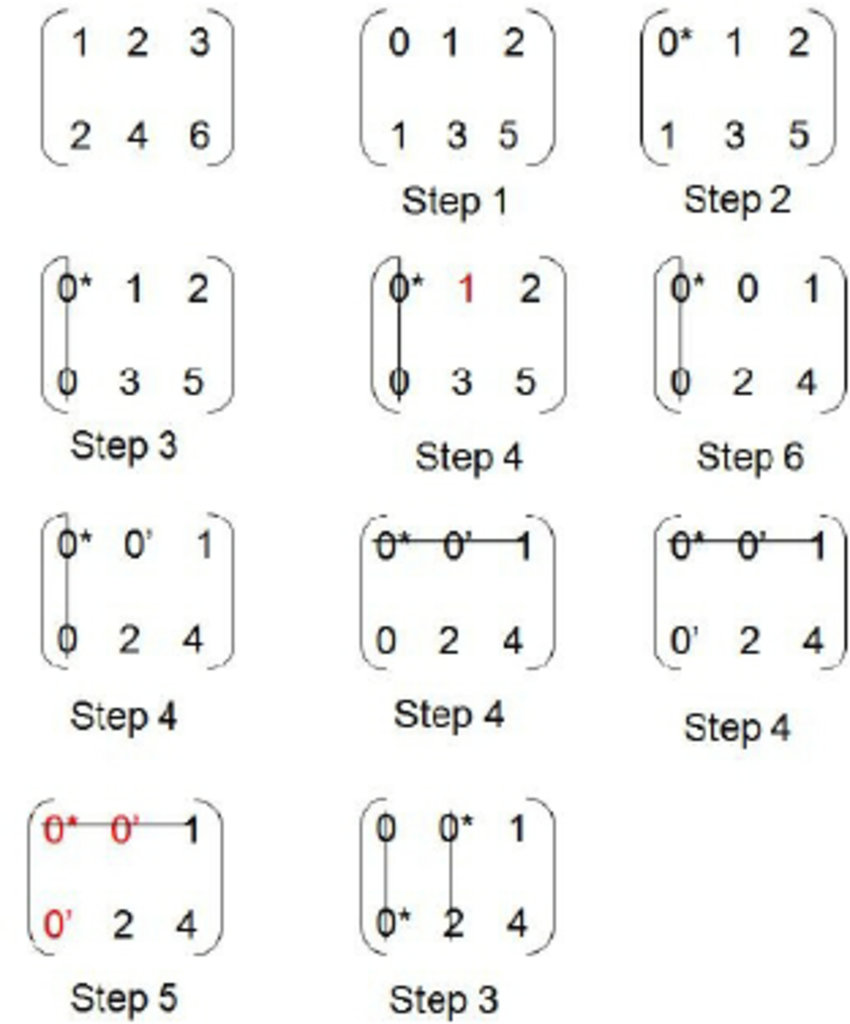
\includegraphics[scale=0.20]{Kuhn-Munkres-example.png}}
        \end{figure}
\end{frame}

\begin{frame}
    \frametitle{Čas na naključnih matrikah}
    \begin{block}{}
        Vzemimo $1000$ matrik velikost $10 \times 10$ z elementi iz enakomerne 
        porazdelitve s spodnjo mejo $1$ in zgornjo mejo $10$.
        Poženemo madžarsko metodo za problem minimalne cene in dobimo:
        \begin{itemize}
            \item povprečen čas: $0.00236$
            \item max čas: $0.012192$
            \item min čas: $0.000561$
        \end{itemize}
    \end{block}
    \begin{figure}[htbp]
        \centerline{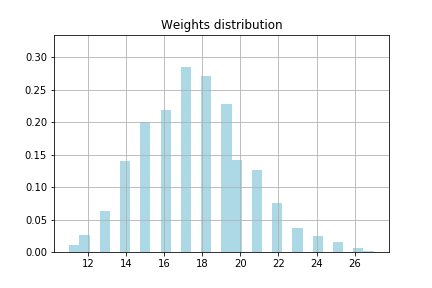
\includegraphics[scale=0.40]{picture1011min.png}}
    \end{figure}
\end{frame}

\begin{frame}
    \frametitle{Čas na naključnih matrikah}
    \begin{block}{}
        Če poženemo na istih matrikah madžarsko metodo za problem maksimalne cene oz.
        profita, se čas izvedbe algoritma ne spremeni.
        \begin{itemize}
            \item povprečen čas: $0.00236$
            \item max čas: $0.011481$
            \item min čas: $0.000614$
        \end{itemize}
    \end{block}
    \begin{figure}[htbp]
        \centerline{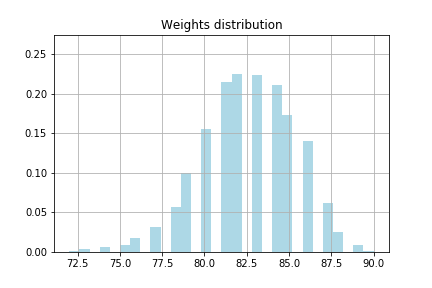
\includegraphics[scale=0.40]{picture1011max.png}}
    \end{figure}
\end{frame}

\begin{frame}
    \frametitle{Čas na naključnih matrikah}
    \begin{block}{}
        Povečajmo velikost matrike na $100 \times 100$, ostale parametre pa pustimo enake.
        \begin{itemize}
            \item povprečen čas: $1.627091$
            \item max čas: $2.503931$
            \item min čas: $0.536118$
        \end{itemize}
    \end{block}
    \begin{figure}[htbp]
        \centerline{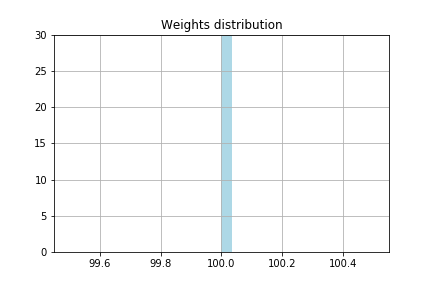
\includegraphics[scale=0.40]{picture111min.png}}
    \end{figure}
\end{frame}

\begin{frame}
    \frametitle{Čas na naključnih matrikah}
    \begin{block}{}
        Povečajmo še interval enakomerne porazdelitve na $[1, 1000]$
        \begin{itemize}
            \item povprečen čas: $2.385538$
            \item max čas: $3.534982$
            \item min čas: $1.405796$
        \end{itemize}
    \end{block}
    \begin{figure}[htbp]
        \centerline{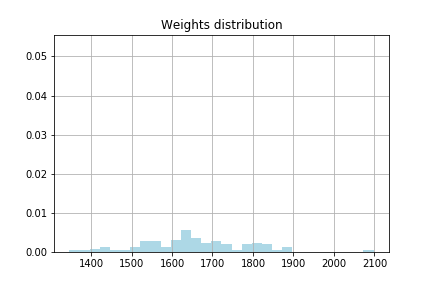
\includegraphics[scale=0.40]{picture1101min.png}}
    \end{figure}
\end{frame}

\begin{frame}
    \frametitle{Čas v odvisnosti od velikosti}
    \begin{block}{}
        Graf, ki prikaže kako je povprečen čas izvedbe algoritma odvisen od velikosti matrike cen.
    \end{block}
    \begin{figure}[htbp]
        \centerline{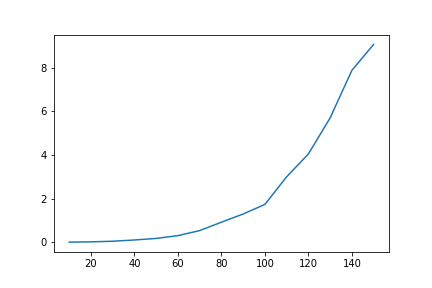
\includegraphics[scale=0.40]{algorithm_time.png}}
    \end{figure}
\end{frame}

\begin{frame}
    \frametitle{Normalna porazdelitev}
    \begin{block}{}
        $1000$ normalno porazdeljenih $10 \times 10$ matrik z povprečjem $3$ in
        standardno deviacijo $1$
        \begin{itemize}
            \item povprečen čas: $0.003358$
            \item max čas: $0.008787$
            \item min čas: $0.000778$
        \end{itemize}
    \end{block}
    \begin{figure}[htbp]
        \centerline{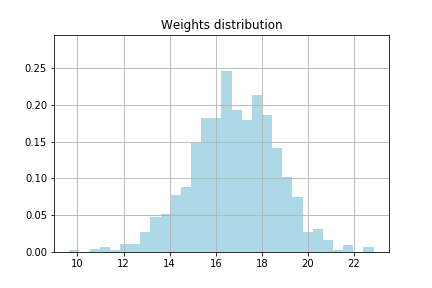
\includegraphics[scale=0.40]{picture1004min.png}}
    \end{figure}
\end{frame}

\begin{frame}
    \frametitle{Normalna porazdelitev}
    \begin{block}{}
        $100$ normalno porazdeljenih $100 \times 100$ matrik z povprečjem $100$ in
        standardno deviacijo $20$
        \begin{itemize}
            \item povprečen čas: $5.220417$
            \item max čas: $11.904078$
            \item min čas: $3.463367$
        \end{itemize}
    \end{block}
    \begin{figure}[htbp]
        \centerline{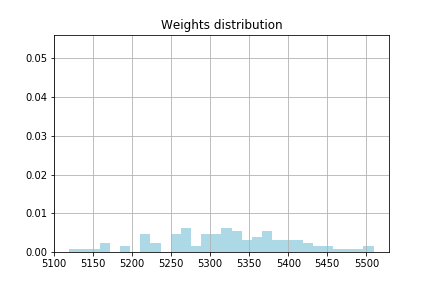
\includegraphics[scale=0.40]{picture220min.png}}
    \end{figure}
\end{frame}

\begin{frame}
    \frametitle{Normalna porazdelitev}
    \begin{block}{}
        $100$ normalno porazdeljenih $100 \times 100$ matrik z povprečjem $100$ in
        standardno deviacijo $20$
        \begin{itemize}
            \item povprečen čas: $5.220417$
            \item max čas: $11.904078$
            \item min čas: $3.463367$
        \end{itemize}
    \end{block}
    \begin{figure}[htbp]
        \centerline{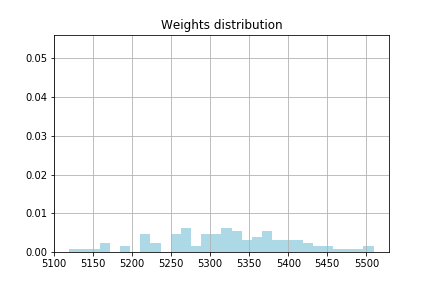
\includegraphics[scale=0.40]{picture220min.png}}
    \end{figure}
\end{frame}

\begin{frame}
    \frametitle{Beta porazdelitev}
    \begin{block}{}
        $1000$ beta porazdeljenih $100 \times 100$ matrik z $\alpha = 0.5$ in
        $\beta = 0.5$ in \textit{min} problemom.
        \begin{itemize}
            \item povprečen čas: $0.003324$
            \item max čas: $0.063679$
            \item min čas: $0.000769$
        \end{itemize}
    \end{block}
    \begin{figure}[htbp]
        \centerline{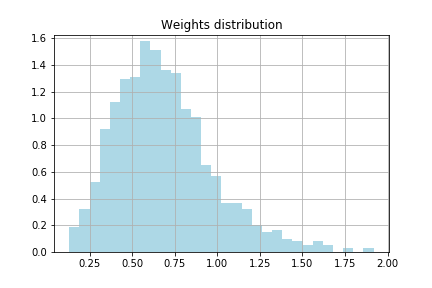
\includegraphics[scale=0.40]{picture1004minbeta.png}}
    \end{figure}
\end{frame}

\begin{frame}
    \frametitle{Beta porazdelitev}
    \begin{block}{}
        $1000$ beta porazdeljenih $100 \times 100$ matrik z $\alpha = 0.5$ in
        $\beta = 0.5$ in \textit{max} problemom.
        \begin{itemize}
            \item povprečen čas: $0.003218$
            \item max čas: $0.009227$
            \item min čas: $0.000797$
        \end{itemize}
    \end{block}
    \begin{figure}[htbp]
        \centerline{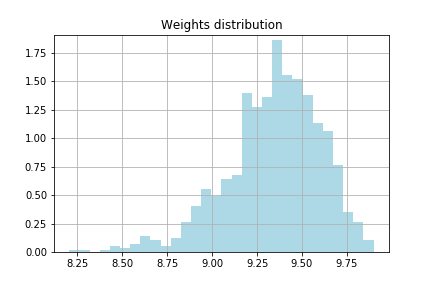
\includegraphics[scale=0.40]{picture1004maxbeta.png}}
    \end{figure}
\end{frame}


\end{document}
